\section{Objetos} \label{sec:objetos}

Para esta implementación, creamos 4 tipos de objetos básicos representables en nuestra escena:

\begin{itemize}
    \item Esferas
    \item \textbf{Planos}
    \item \textbf{Cajas}
    \item \textbf{Triángulos}
\end{itemize}

A continuación explicaremos brevemente la implementación de aquellos que están en negrita, ya que
el resto podemos encontrarlos en la guía de Shirley.

\subsection{Planos}\label{subsec:planos}

Representamos a un plano como un par de 2 vectores, uno apuntando a un punto de referencia ($P$) que
pertenezca al plano, y uno perpendicular al plano ($N$).
Consideremos un rayo $r(t) = O + t D$, donde $O$ es el origen y $D$ es la dirección del mismo,
entonces la intersección entre el plano y el rayo se da en $t = \frac{(P - O) \cdot N}{D \cdot N}$.
Notar que la intersección se da siempre y cuando $D \cdot N$ no de 0, es decir, el rayo no sea
paralelo al plano.

\begin{figure}[H]
    \centering
    \begin{subfigure}{0.45\linewidth}
        \centering
        
\includegraphics[width=\textwidth]{imgs/escena_plano}
        \caption{Render del plano x=0}
        \label{fig:render_plano_x0}
    \end{subfigure}
    \begin{subfigure}{0.45\linewidth}
        \centering
        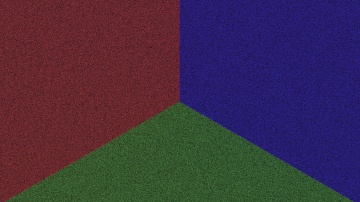
\includegraphics[width=\textwidth]{imgs/escena_3_planos}
        \caption{Render de los planos x=0, y=0 y z=0}
        \label{fig:render_planos_0}
    \end{subfigure}
    \caption{Planos}
\end{figure}

En la figura~\ref{fig:render_plano_x0} vemos el plano $x=0$ en verde, mientras que en la
figura~\ref{fig:render_planos_0} vemos los 3 planos $x=0$, $y=0$ y $z=0$ en rojo, verde y azul
respectivamente.

\subsection{Cajas} \label{subsec:cajas}

Las cajas las implementamos con 6 planos, cada uno representando a la cara correspondiente.
Para que la implementación sea simple, decidimos que las caras estarían alineadas a los ejes
cartesianos.
Para verificar si un rayo colisiona con la caja, recorremos cada cara y calculamos el punto en el
que el rayo y el plano se intersecan.
Si este punto pertenece a alguna cara de la caja, lo consideramos para calcular el punto final,
que sería el más cercano.
Si ningún punto pertenece a una cara de la caja, consideramos que no hay colisión.

Las cajas se definen por 2 vertices opuestos, el que tiene las coordenadas menores y el que tiene
las coordenadas mayores.
En la figura~\ref{fig:escena_caja_vertices} podemos ver una caja con un vértice rojo $P=(0,.1,0)$
y un vértice amarillo $Q=(1,1.1,1)$.

\begin{figure}[H]
    \centering
    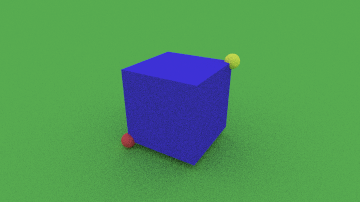
\includegraphics[width=.9\textwidth]{imgs/escena_caja_vertices}
    \caption{Render de una caja, indicando los vertices que lo identifican}
    \label{fig:escena_caja_vertices}
\end{figure}

\subsection{Triángulos} \label{subsec:triangulos}

Los triángulos los definimos con 3 vertices, $P_0, P_1$ y $P_2$.
Para calcular la intersección con un rayo, primero calculamos la intersección con el plano que
contiene al triangulo y luego verificamos si este punto $P$ se encuentra dentro del triangulo.
Para hacer esto, calculamos las normales de los triángulos $P_0 P_1 P$, $P_1 P_2 P$ y $P_2 P_0 P$.
Si estas normales apuntan hacia el mismo lado que la normal del triangulo original, entonces el
punto $P$ se encuentra dentro.

\begin{figure}[H]
    \centering
    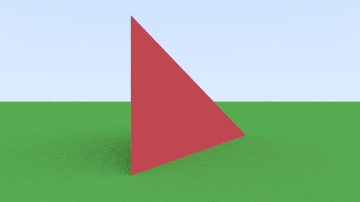
\includegraphics[width=.9\textwidth]{imgs/escena_triangulo}
    \caption{Render de un triángulo}
    \label{fig:escena_triangulo}
\end{figure}

En la figura~\ref{fig:escena_triangulo} vemos un triangulo de vertices $(1,0,0)$, $(0,1,0)$ y $
(0,0,1)$.